\documentclass[a4paper,
12pt,
BCOR12mm,
]{scrartcl}
%scrreport
\usepackage[ngerman]{babel}
\usepackage[utf8]{inputenc}
\usepackage[T1]{fontenc}
\usepackage{url}
\usepackage[pdftex]{graphicx}
\usepackage{listingsutf8}
\usepackage{grffile}
\usepackage{epstopdf}
\usepackage{subfigure}
\usepackage{multicol}
\usepackage{fullpage}
% lstlisting settings
\lstset{
showspaces=false,
breaklines=true,
breakindent=0pt,
frame=single,
language=erlang,
extendedchars=true,
inputencoding=utf8/latin1,
identifierstyle=\ttfamily,
basicstyle=\tiny,
numbers=left,
numberstyle=\tiny,
}

\usepackage{amsmath}
\usepackage{amsfonts}
\usepackage{amssymb}
% \usepackage{mathtools} not installed?
\usepackage{stmaryrd}
\usepackage{graphicx}
\usepackage[ngerman]{babel}
\usepackage{algpseudocode}

\usepackage{hyperref}

\usepackage{color}

\usepackage{paralist} % inline list

% enhanced enumerate 
% see http://texblog.wordpress.com/2008/10/16/lists-enumerate-itemize-description-and-how-to-change-them/
\usepackage{enumerate}

% i hate the fat blob..
\renewcommand{\labelitemi}{\guilsinglright}

\usepackage[thmmarks,amsmath,amsthm]{ntheorem}

\theorempreskipamount 14pt
\theorempostskipamount 12pt
\theoremstyle{break}
\theoremheaderfont{\scshape \smallskip}
\theorembodyfont{\normalfont}
\newtheorem{defi}{Definition}[subsection]

% vektoren durch $\mat{1 \\ 2 \\ 3}$
\def\mat#1{\left(\begin{array}{cccccc}#1\end{array}\right)}

% framebox
\def\framebox#1{\fbox{\begin{minipage}{0.8\textwidth}{#1}\end{minipage}}\\}

% questionbox
\usepackage{fancybox}
\def\questionbox#1{\shadowbox{\begin{minipage}{0.8\textwidth}{ {\Huge ?} \color{red}{#1}}\end{minipage}}\\}
\def\warningbox#1{\shadowbox{\begin{minipage}{0.8\textwidth}{ {\Huge !} \color{blue}{#1}}\end{minipage}}\\}

% condensed lists
\usepackage{mdwlist}

\usepackage{verbatim}

% floor funktion
\def\floor#1{\left\lfloor #1 \right\rfloor}

\newtheorem{beh}{Behauptung}
\newtheorem{bew}{Beweis}
\newtheorem{afg}{Aufgabe}
\newtheorem{lsg}{Lösung}
\newtheorem{lem}{Lemma}[subsection]
\newtheorem{bsp}{Beispiel}[subsection]
\newtheorem{satz}{Satz}[subsection]
\newtheorem{define}{Definition}
\theoremsymbol{$\square$}

\title{APUVS, Blatt 10}
\author{Jan Fajerski and Kai Warncke and Magnus Müller}

\begin{document}
% NOTE: compile with pdflatex --shell-escape main.tex

\maketitle 

\section*{Aufgabe 10.1}
\begin{itemize}
  \item[1] Beide Transaktionen können validiert werden, da U ein leeres Readset
    hat. i=55; j=66
  \item[2] T wird abgebrochen, da das Readset von T (enthält i) mit dem Writeset
    von U überlappt. T muss also davon ausgehen, einen inkonsistenten Wert
    gelesen zu haben. U wird validiert. i=55; j=66
  \item Beide Transaktionen werden validiert, da U zum Zeitpunkt der Validierung
    von T ein leeres Writeset besitzt. i=55; j=66
  \item T wird abgebrochen, da das Readset von T mit dem Writeset von U
    überlappt. T könnte also einen inkonsistenen Wert gelesen haben und wird
    aufgefordert sich abzubrechen. i=55; j=66
\end{itemize}

\section*{Aufgabe 10.2}
 Zum Start des Programms die Funktion \verb+testcr(N)+ aufrufen, wobei N die Anzahl der
 gewünschten Prozesse ist. 
 \lstinputlisting{../src/changrob.erl}
 \lstinputlisting{../src/collector.erl}
 \lstinputlisting{../src/test.erl}

 \pagebreak

 \begin{figure}
   \begin{center}
     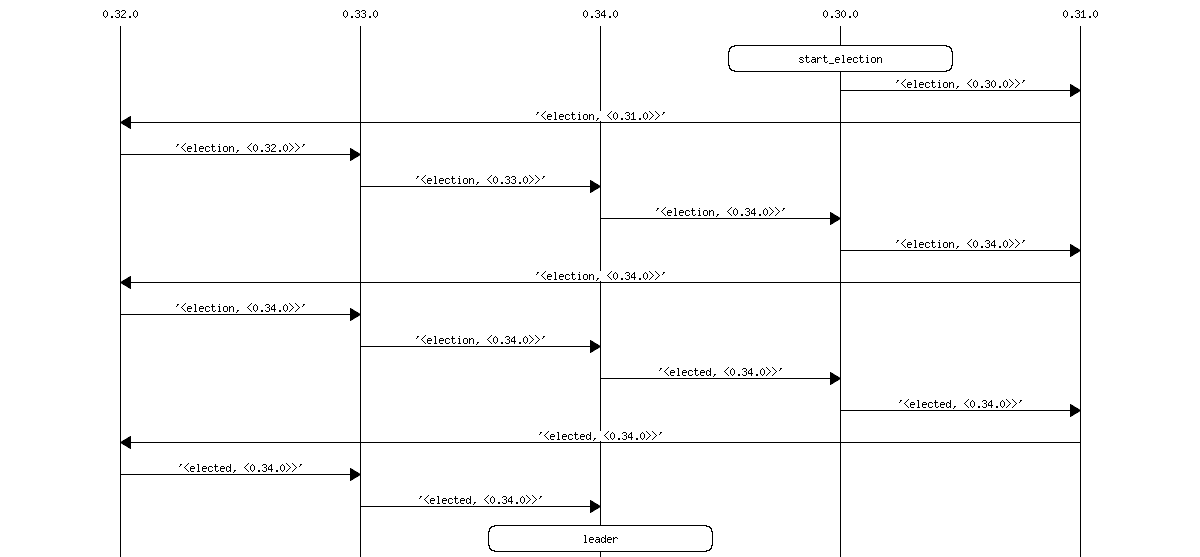
\includegraphics[scale=0.4]{../src/msc/single_election_at_0.30.0.png}
   \end{center}
   \caption{Wahlstart bei 0.30.0; Anzahl der Nachrichten: 14}
   \label{fig:s_30}
 \end{figure}

 \begin{figure}
   \begin{center}
     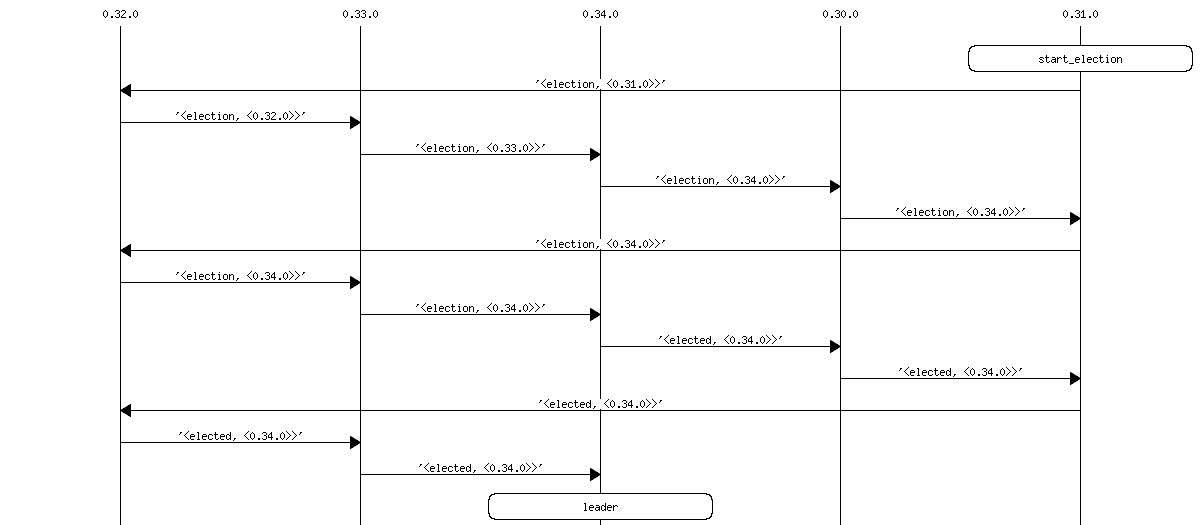
\includegraphics[scale=0.4]{../src/msc/single_election_at_0.31.0.png}
   \end{center}
   \caption{Wahlstart bei 0.31.0; Anzahl der Nachrichten: 13}
   \label{fig:s_31}
 \end{figure}

 \begin{figure}
   \begin{center}
     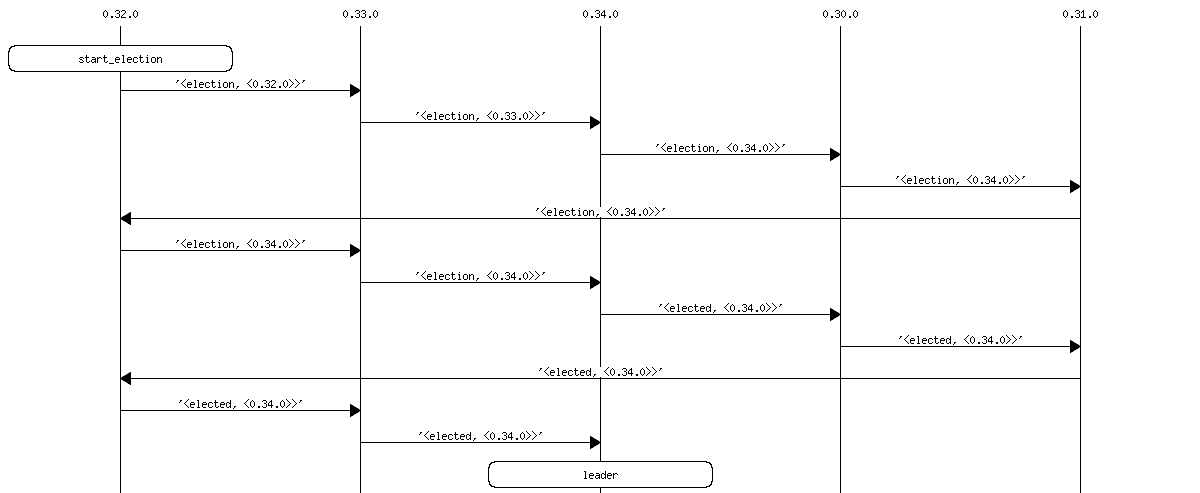
\includegraphics[scale=0.4]{../src/msc/single_election_at_0.32.0.png}
   \end{center}
   \caption{Wahlstart bei 0.32.0; Anzahl der Nachrichten: 12}
   \label{fig:s_32}
 \end{figure}

 \begin{figure}
   \begin{center}
     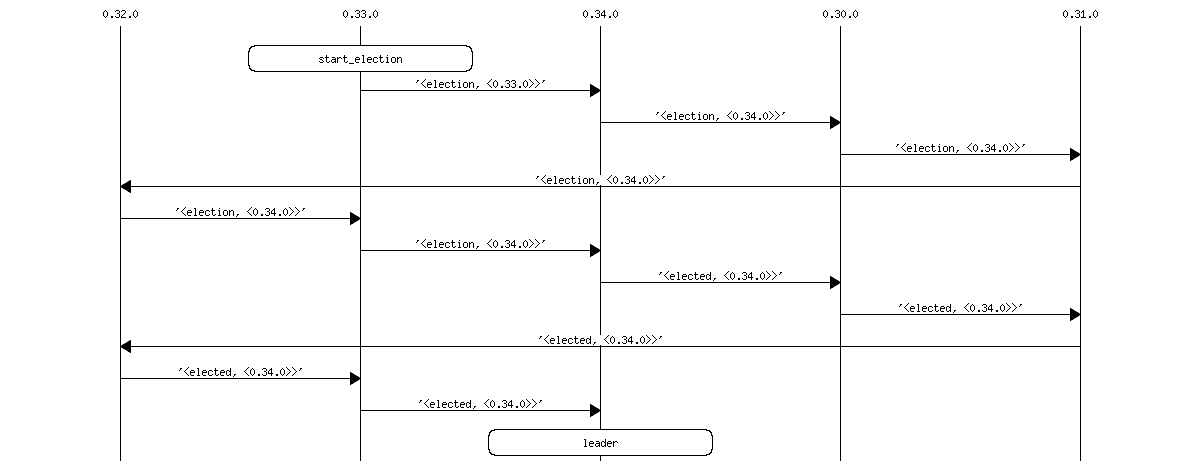
\includegraphics[scale=0.4]{../src/msc/single_election_at_0.33.0.png}
   \end{center}
   \caption{Wahlstart bei 0.33.0; Anzahl der Nachrichten: 11}
   \label{fig:s_33}
 \end{figure}

 \begin{figure}
   \begin{center}
     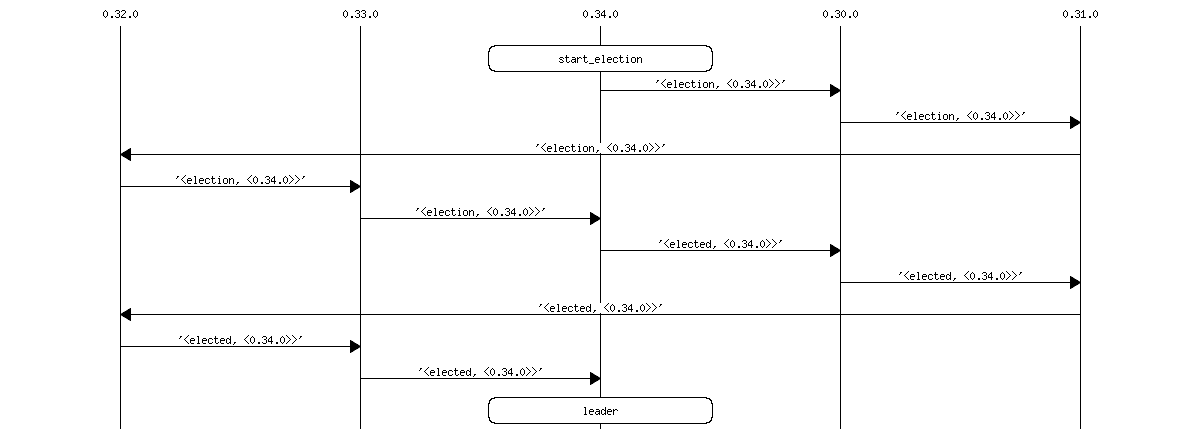
\includegraphics[scale=0.4]{../src/msc/single_election_at_0.34.0.png}
   \end{center}
   \caption{Wahlstart bei 0.34.0; Anzahl der Nachrichten: 10}
   \label{fig:s_34}
 \end{figure}

 \begin{figure}
   \begin{center}
     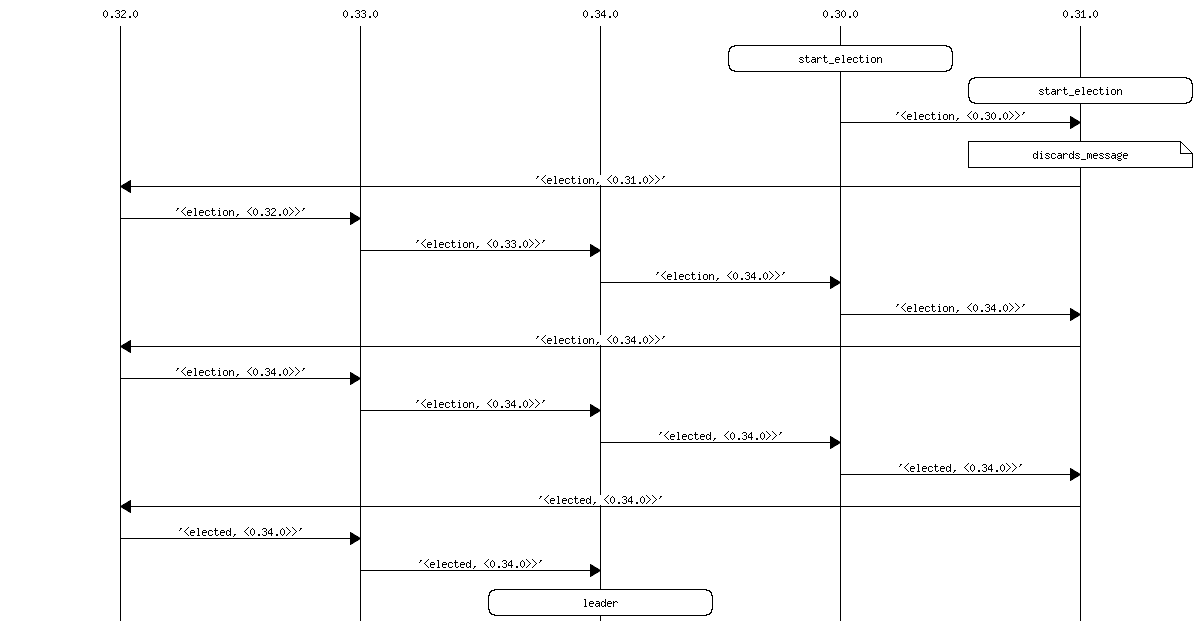
\includegraphics[scale=0.4]{../src/msc/concurrent_with_0.30.00.31.0.png}
   \end{center}
   \caption{Wahlstart bei 0.30.0 und 0.31.0; Anzahl der Nachrichten: 14}
   \label{fig:s_3031}
 \end{figure}

 \begin{figure}
   \begin{center}
     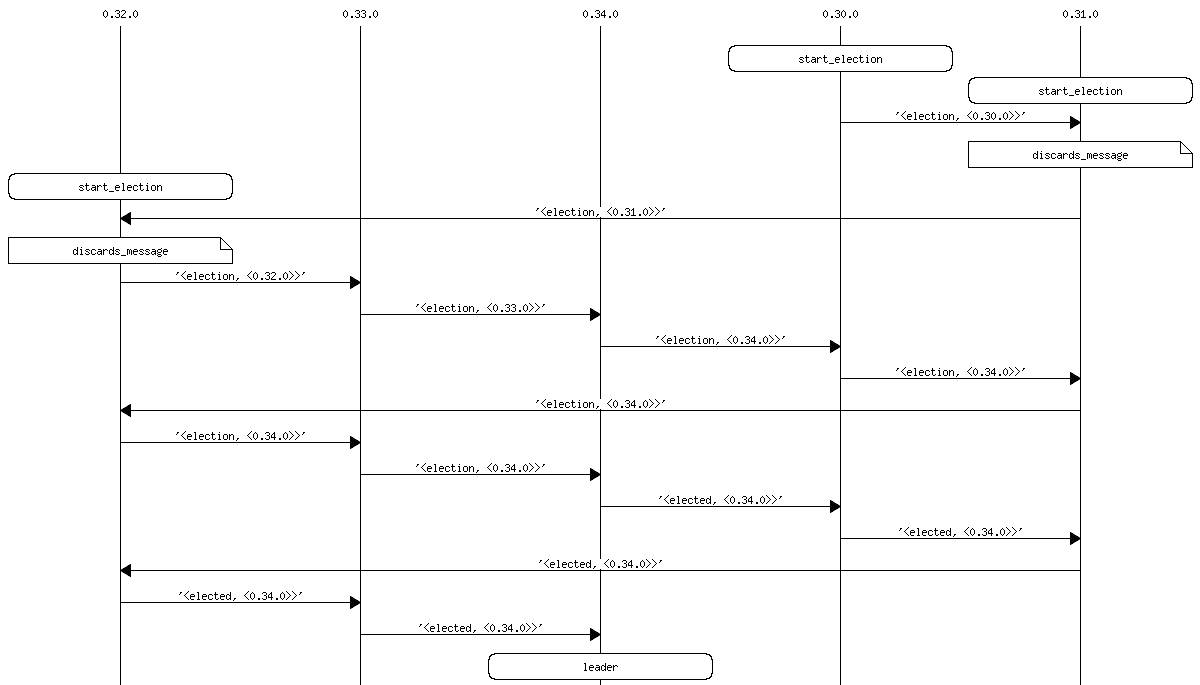
\includegraphics[scale=0.4]{../src/msc/concurrent_with_0.30.00.31.00.32.0.png}
   \end{center}
   \caption{Wahlstart bei 0.30.0, 0.31.0 und 0.32.0; Anzahl der Nachrichten: 14}
   \label{fig:s_303132}
 \end{figure}

 \begin{figure}
   \begin{center}
     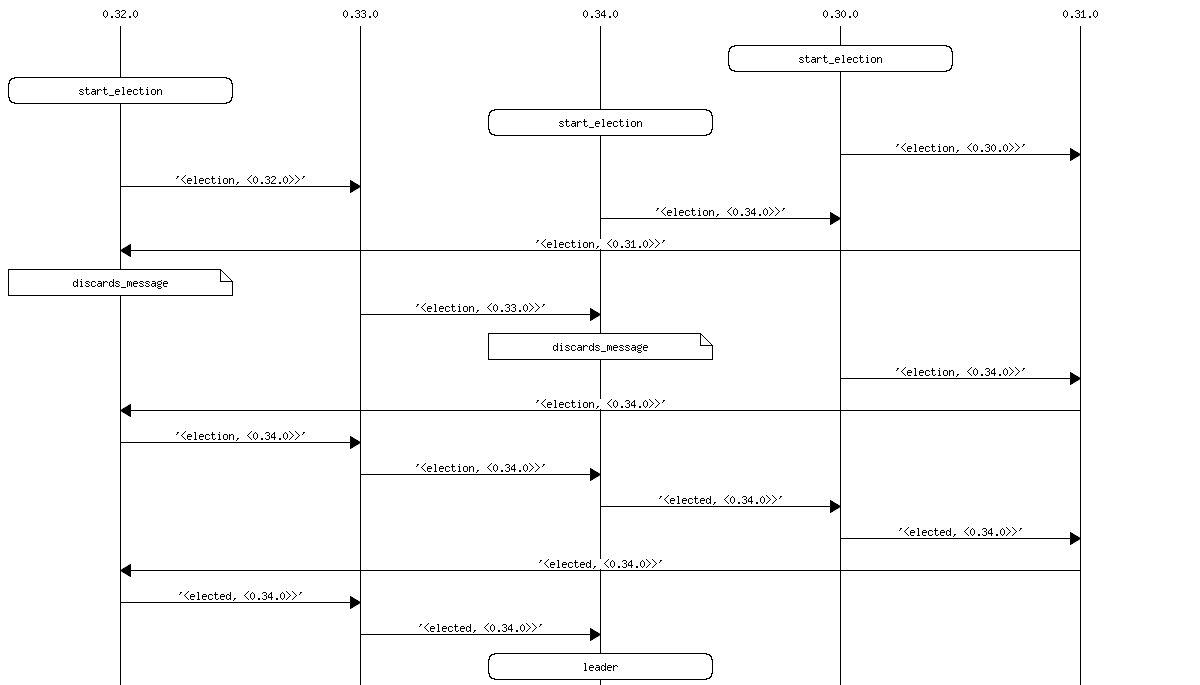
\includegraphics[scale=0.4]{../src/msc/concurrent_with_0.30.00.32.00.34.0.png}
   \end{center}
   \caption{Wahlstart bei 0.30.0, 0.32.0 und 0.34.0; Anzahl der Nachrichten: 14}
   \label{fig:s_303234}
 \end{figure}

 \begin{figure}
   \begin{center}
     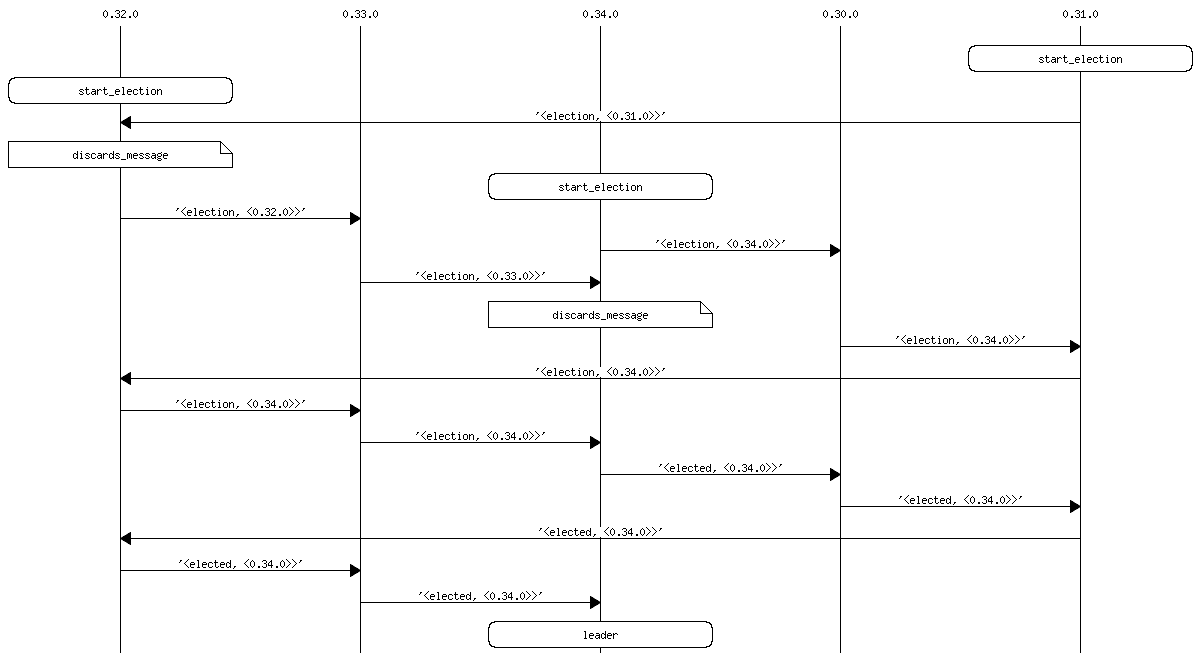
\includegraphics[scale=0.4]{../src/msc/concurrent_with_0.31.00.32.00.34.0.png}
   \end{center}
   \caption{Wahlstart bei 0.31.0, 0.32.0 und 0.34.0; Anzahl der Nachrichten: 13}
   \label{fig:s_313234}
 \end{figure}

\end{document}
